\documentclass[12pt]{report}

% Language and encoding
\usepackage[english]{babel}

% Font packages
\usepackage{fontspec}
\setmainfont{Times New Roman}
\setsansfont{Arial}
\setmonofont{Courier New}

% Math font setup
\usepackage{unicode-math}
\setmathfont{XITS Math}       % Or use another font like 'Latin Modern Math'

% Page margins
\usepackage{geometry}
\geometry{a4paper, left=1.5in, right=1in, top=1in, bottom=1in}
\usepackage{amsmath,graphicx, xcolor}
\usepackage{enumitem}

\usepackage{etoolbox}
\apptocmd{\biburlsetup}{\Urlmuskip=0mu plus 1mu\relax}{}{}

% \usepackage{url}
% \def\UrlBreaks{\do\/\do-}

\usepackage[hyphens]{url}
\usepackage{xurl}  % Allows line breaks in URLs
\usepackage{hyperref}
\hypersetup{
    colorlinks=true,
    linkcolor=blue,
    filecolor=magenta,      
    urlcolor=blue,
    pdftitle={Overleaf Example},
    pdfpagemode=FullScreen,
    }

% Line spacing
\usepackage{setspace}
\doublespacing  % Use \onehalfspacing for 1.5 line spacing

% For figures and tables
\usepackage{graphicx}
\usepackage{caption}
\usepackage{subcaption}
\usepackage{booktabs} % For better table lines
\usepackage{tabularx}
\usepackage{array}
\usepackage{longtable} % For long tables
\usepackage{multirow} % For multi-row cells in tables
\usepackage{float} % For placing figures and tables

% For references
\usepackage{url} % For clickable URLs in the bibliography
% \usepackage{cite}
\usepackage{csquotes}         % Add csquotes for proper quotation support
\usepackage[
    backend=biber,
    style=ieee,
    url=true,
    doi=false,
    isbn=false,
    eprint=false,
    maxcitenames=2,
    maxbibnames=6
]{biblatex}
\addbibresource{references.bib}

\usepackage{lipsum} % For dummy text


\title{A Retrieval-Augmented Generation Approach with Fine-Tuned SahabatAI for Indonesian Consular Chatbot
}
\author{Fathur Rohman}
\date{May, 2025}

\begin{document}

\sloppy
\begin{titlepage}
  \begin{center}
    \vspace*{2cm} % Adjust vertical spacing as needed

    {\LARGE \textbf{A Retrieval-Augmented Generation Approach with Fine-Tuned SahabatAI for Indonesian Consular Chatbot}} \\[1.5cm]

    \textbf{Fathur Rohman} \\[1.5cm]

    \vspace{5cm} % Additional space to move the university name down
    \textbf{President University} \\[0.5em]
    Informatics Study Program \\[0.5em]
    Master of Science in Information Technology \\[0.5em]
    \textbf{Thesis Proposal} \\[0.5em]
    \textbf{2025} \\[0.5em]
    \textbf{Thesis Supervisor:} \\[0.5em]
    \textbf{Dr. Fulan, S.T., M.T.} \\[0.5em]
    \textbf{Thesis Co-Supervisor:} \\[0.5em]    
    \textbf{Dr. Fulana, S.T., M.T.} \\[0.5em]
  \end{center}
\end{titlepage}

\begin{center}
  \textbf{Abstract}
\end{center}
\begin{spacing}{1.5} % Use 1.5 line spacing for the abstract

Providing good consular services to citizen abroad is crucial for the Indonesian government. Ministry of Foreign Affairs (Kemenlu) has launched digital platforms like "Peduli WNI", "Safe Travel", and the "SARI" chatbot.
while SARI is focused on migrant workers, it may not cover all consular services queries. 
This research aims to develop a Question Answering (QA) system using a Retrieval-Augmented Generation (RAG) approach with a fine-tuned SahabatAI model(base on Gemma2 and llama3) to answer questions related to Indonesian consular services. 
The method focuses on applying Parameter-Efficient Fine-Tuning (PEFT) to adapt SahabatAI for consular topics, implementing a Retrieval-Augmented Generation (RAG) system with SahabatAI as the response generator, and building a specialized knowledge base from official MoFA sources.
The evaluation will focus on how well the system retrieves information, the quality of generated answers (accuracy and relevance), and overall performance.
The expected outcome is a robust QA system that can provide accurate and timely information to Indonesian citizens seeking consular services.

\textbf{Keywords:} Consular Services, SahabatAI Fine-Tuning, Retrieval-Augmented Generation, Fine-Tuning (RAG), Question Answering (QA) System, Public Service Automation.
\end{spacing}


\newpage

% Table of Contents
\tableofcontents
\newpage

% List of Figures (if applicable)
\listoffigures
\newpage

% List of Tables (if applicable)
\listoftables
\newpage

% Chapter 1: Introduction
\chapter{Introduction}
\section{Background}

Consular services represent a cornerstone of a nation's support for its citizens abroad. These services, which include the issuance of passports and visas, provision of emergency assistance, facilitation of self-reporting for citizens residing overseas, and management of case reports, are vital for ensuring the safety, well-being, and legal standing of individuals in foreign territories~\cite{UU37_1999,Keppres108_2003}. The Indonesian Ministry of Foreign Affairs (MoFA) is tasked with serving a substantial global diaspora and a large number of citizens traveling internationally~\cite{KPU301_2024}, which underscores the necessity for highly
efficient, accessible, and responsive support mechanisms.

In response to these demands, the Indonesian MoFA has proactively embraced digital transformation to enhance its consular service delivery~\cite{Tempo_AI_Kemlu}. This commitment is evident in its existing digital ecosystem:
% maksimum width 15.65 cm untuk content
\begin{table}[htbp]
    \centering
    \caption{Overview of Consular Service Platforms}
    \resizebox{\textwidth}{!}{
        \begin{tabular}{|p{2cm}|p{2cm}|p{5cm}|p{2cm}|p{2.5cm}|}
        \hline
        \textbf{Platform Name} & \textbf{Type} & \textbf{Key Features} & \textbf{Target Users} & \textbf{Reported AI/Technology Used} \\ 
        \hline
        Portal Peduli WNI & Web-portal & Lapor Diri (Self-Reporting), Pelayanan Kekonsuleran (Consular Services), and Pengaduan Kasus (Case Reporting) & Indonesian citizens abroad & Web-based platform \\ 
        \hline
        Safe Travel & Mobile App & Trip registration, country-specific information, notifications, emergency assistance (location sharing, video recording) & Indonesian citizens traveling abroad for short trips & Mobile application \\ 
        \hline
        SARI (Sahabat Artifisial Migran Indonesia) & Chatbot & designed capacity for empathetic responses & Indonesian female migrant workers abroad & AI-powered chatbot, NLP, integrated with Safe Travel \\ 
        \hline
    \end{tabular}
    }
\end{table}

\begin{itemize}
    \item \textbf{Peduli WNI:} This web-based platform serves as a central hub for Indonesian citizens abroad, offering critical features such as Lapor Diri (Self-Reporting), Pelayanan Kekonsuleran (Consular Services), and Pengaduan Kasus (Case Reporting). The portal has significantly streamlined processes that previously necessitated physical visits to Indonesian embassies or consulates, allowing services to be accessed online with internet connectivity~\cite{PeduliWNI}.
    \item \textbf{Safe Travel:} A mobile application designed for Indonesian citizens undertaking short trips abroad, although it can also be utilized by expatriates. It provides practical country-specific information (e.g., time differences, security conditions, local laws and customs, immigration requirements, health services at Indonesian missions), travel registration, notifications (appeals, advice, warnings), and crucial emergency assistance features. In critical situations, users can send their location, record video, and contact the nearest Indonesian mission.
    \item \textbf{SARI Chatbot:} This AI-powered chatbot represents a significant step towards leveraging advanced technology for citizen protection. Developed in collaboration with UN Women, SARI is specifically tailored to assist and protect Indonesian female migrant workers from potential violence and exploitation. Integrated within the Safe Travel application, SARI aims to deliver accessible, unbiased, and non-discriminatory information. A key feature is its designed capacity for empathetic responses. The launch of SARI underscores MoFA's commitment to "digital empathy" and delivering excellent service and protection, particularly for vulnerable groups~\cite{kemlu2025chatbot}.
\end{itemize}

The global landscape of public servce delivery is increasingly being reshaped by andvancements in artificial intelligence (AI), particularly Large Language Models (LLMs) and Retrieval-Augmented Generation (RAG) techniques. These technologies offer transformative potential including 24/7 citizen assistance, the capacity to handle complex and nuanced queries, multilingual support, and the ability to personalize interactions, thereby enhancing the efficiency and effectiveness of government services.

A recent development in Indonesia's AI journey is SahabatAI, a large language model (LLM) fine-tuned for Indonesian language tasks~\cite{gemma2_sahabat_ai_v1_instruct}. SahabatAI is collaborative initiative by Indosat Ooredo Hutchison and GoTo Group based on the Gemma2~\cite{gemma2_sahabat_ai_v1_instruct} and llama3 architecture~\cite{llama3_sahabat_ai_v1_instruct}, which has been trained on a diverse range of Indonesian text data comprising over 640,000 instruction-completion pairs, covering Bahasa Indonesia, Javanese, and Sundanese, with plans to include other regional languages like Batak and Balinese. The core objectives of SahabatAI include promoting linguistic diversity, fostering AI sovereignty for Indonesia, and enabling seamless business-to-government (B2G) and business-to-business (B2B) interactions to significantly enhance the quality and accessibility of government services. Potential use cases for SahabatAI in the public sector include simplifying applications for the national identity card (KTP), demystifying taxation processes, and streamlining procuderes for official document changes related to live events such as marriage ore relocation.

The newly existance of SahabatAI as open-source LLM, extensively trained on Indonesian text data, presents relevant technological foundation for this thesis. Developing an LLM from scratch is a complex and resource-intensive endeavor, requiring substantial computational power and extensive datasets, far exceeding the scope of a Master's thesis. By leveraging SahabatAI, this research can focus on fine-tuning the model for specific tasks, such as consular services, while also exploring the integration of RAG techniques to enhance the system's performance and responsiveness.

\section{State of the Art}

Large Language Models (LLMs), primarily based on the Transformer architecture, have revolutionized natural language processing (NLP) and artificial intelligence (AI)~\cite{NIPS2017_3f5ee243}. it has demonstrated capabilities in various tasks, including text generation, translation, summarization, and question answering. This makes them suitable for complex Question Answering (QA) tasks, where they can interpret user queries and generate relevant, coherent responses based on their vast pre-trained knowledge or context provided at inference time~\cite{jm3}. 

Retrieval-Augmented Generation (RAG) is a techniques developed to enhance the capabilities of LLMs, particularly in knowledge-intensive tasks~\cite{NEURIPS2020_6b493230}. RAG architectures connect LLMs with external, often dynamic, knowledge sources, allowing them to retrieve relevant information from a database or document corpus before generating a response. This approach addresses the limitations of LLMs, such as their fixed knowledge base and potential inaccuracies in generated content~\cite{gupta2024comprehensivesurveyretrievalaugmentedgeneration}. By integrating retrieval mechanisms, RAG systems can provide more accurate and contextually relevant answers, especially in domains where up-to-date information is crucial.
By retrieving relevant information from these sources and providing it as context to the LLM during answer generation, RAG mitigates common LLM limitations, such as hallucinations and outdated knowledge. This is particularly important in dynamic fields like consular services, where information can change over time and needs to adhere to current laws and regulations.

The application of AI in consular services is growing trend globally~\cite{govnet2025}. Governments are increasingly exploring AI-powered solutions, including chatbots for handlung frequently asked questions, assisting with visa applications, and providing real-time information to citizens. For instance, Singapore's GovTech Agency has deployed AI chatbots accross various government departments, leading significant reduce in call center workloads and faster response times for citizen inquiries~\cite{govsgvica2025}.
Similarly, the U.S. Department of State has outlined  plans to use AI for various consular function, including passport photo quality assessment, analysis of customer feedback, AI-driven translation services, and enhanced search and chatbot systems for its Travel.State.Gov website~\cite{usdosai2025}.
These examples highlight a global shift towards leveraging AI to make consular services more efficient, accessible, and responsive to citizen needs. Other relevant works include general AI Principles~\cite{molaee2025}, and AI applications in diplomacy~\cite{mostafaei2025}.

\section{Gap Analysis}

Despite the Indonesian MoFA's commendable efforts in digital transformation like the development of the "Peduli WNI" platform, "Safe Travel" application, and SARI chatbot, several gaps and opportunities remain for enhancing consular services delivery through AI. 

While the existing platforms provide valuable services, they may not comprehensively address all consular queries, particularly those related to specific legal or procedural matters. The SARI chatbot, though an innovative AI application, is specifically designed to support Indonesian female migrant workers, focusing on protection against violence and exploitation. This leaves a gap in addressing queries related to other consular services, such as passport renewal procedures, visa regulations for various countries, assistance for lost documents, and general emergency guidance without a dedicated, advanced AI-powered conversational interface. These general queries can be complex, nuanced, and often require synthesizing information from multiple official sources. Current systems may not be equipped to handle such multi-turn conversational interactions or provide comprehensive answers that require understanding implicit user needs. "Peduli WNI" while providing valuable information and transactional services, may not be fully optimized for complex queries. Futhermore, user feedback for existing applications like the "Safe Travel" app has indicated occasional technical issues, such as server connectivity issues and application crashes, suggesting room for improvements in reliability and user experience. Additionally, the current systems may not fully leverage the potential of advanced AI technologies, such as Retrieval-Augmented Generation (RAG) and fine-tuning techniques, to enhance their capabilities.

The advent of SahabatAI, an open-source LLM fine-tuned for Indonesian language tasks, with a strong foundation in Bahasa Indonesian and local dialects like Javanese and Sundanese, presents a unique opportunity to address these gaps. Appliying state-of-the-art RAG techniques in conjunction with SahabatAI model can potentially deliver more accurate, contextually relevant, and up-to-date responses to consular queries than could be achieved with generic LLMs or simple rule-based chatbot technology. The spesific combination of localized LLM like SahabatAI with advanced RAG tailored for Indonesian consular domain remains an underexplored area of research and application.

Moreover, general-purpose LLMs or even generic RAG systems often necessitate significant adaptation to perform optimally in specialized domain such as consular services, This domain is characterized by its unique terminologies, intricate regulations, evolving policies, and diverse user needs context~\cite{karzhevdatacamp2025}. Therefore, fine-tuning SahabatAI to better understand and generate text specific to consular affairs, coupled with the meticulous curation of a dedicated comprehensive consular knowledge base, is crucial for developing an effective and reliable AI assistant.

The existing MoFA digital tools—Peduli WNI (web-based), Safe Travel (mobile app), and SARI (chatbot integrated within Safe Travel)—while individually valuable, operate with some degree of separation in terms of user interface and scope. A sophisticated RAG-based chatbot, as proposed in this research, could serve as a more unified and intelligent front-end. Such a system could potentially integrate information from, or direct users to, these existing platforms, thereby providing a more seamless and comprehensive user experience for a wider range of consular questions. The knowledge base for the RAG system would ideally be constructed by consolidating information from these diverse official MoFA sources, creating a centralized and reliable information backbone for the AI. This approach could improve the discoverability and accessibility of consular information that might currently be distributed across different platforms or document formats.

\section{Research Questions}

The research questions guiding this study are as follows:
\begin{enumerate}
    \item \textbf{RQ1:} How can a RAG system using SahabatAI be designed to accurately and reliably handle various Indonesian consular queries, such as passport renewal, lost documents, and visa regulations?
    \item \textbf{RQ2:} Which PEFT strategies (e.g., QLoRA, instruction tuning) are most effective for adapting SahabatAI to the specific language and information requirements of Indonesian consular queries in a RAG framework?
    \item \textbf{RQ3:} What are the essential components and best practices for developing a high-quality, domain-specific knowledge base and QA dataset for Indonesian consular services to effectively train and evaluate a RAG system?
    \item \textbf{RQ4:} How does the fine-tuned SahabatAI-RAG system perform compared to baseline models (e.g., zero-shot SahabatAI, naive RAG) and existing MoFA chatbot solutions in terms of accuracy, relevance, coherence, and user perceived helpfulness?
    \item \textbf{RQ5:} What practical challenges and ethical considerations arise in deploying an AI-powered consular service assistant, particularly regarding data privacy, bias mitigation, and equitable information access, and how can these be addressed within a six-month Master's thesis?
\end{enumerate}

\section{Research Objectives}

To answer the research questions, this study aims to achieve the following objectives:

\begin{enumerate}
    \item \textbf{RO1:} To design and implement a RAG-based chatbot using SahabatAI to provide accurate and reliable responses to Indonesian consular queries, based on a curated knowledge base of official consular information.
    \item \textbf{RO2:} To implement and evaluate PEFT techniques (e.g., QLoRA) for fine-tuning SahabatAI using a custom Indonesian consular QA dataset, with the goal of improving its domain-specific accuracy and response quality.
    \item \textbf{RO3:} To curate a comprehensive knowledge base from official MoFA resources and develop a representative QA dataset that covers common Indonesian consular service inquiries for training and evaluating the RAG system..
    \item \textbf{RO4:} To assess the performance of the fine-tuned SahabatAI-RAG system against baseline models and MoFA chatbot solutions using automated metrics (e.g., BLEU, ROUGE) and human evaluation to measure accuracy, relevance, coherence, and user perceived helpfulness.
    \item \textbf{RO5:} To identify key ethical challenges, such as data privacy and bias mitigation, in deploying the proposed AI-powered consular assistant and to provide actionable recommendations for addressing these challenges within the scope of a six-month Master's thesis.
\end{enumerate}

\section{Limitations}

This research, while ambitious, will be conducted within the constraints of a six-month Master's thesis timeline. This necessitates a focused scope, particularly in the following areas:

\begin{itemize}
    \item \textbf{Scope of Consular Services:} The primary focus is on Indonesian consular services, including passport renewal, lost documents, and visa regulations.
    \item \textbf{knowledge Base:} The knowledge base will be constructed from publicly available official MoFA resources, with a focus on accuracy and relevance.
    \item \textbf{Language Focus:} While SahabatAI has demonstrated some training in Javanese and Sundanese, the primary focus will be on Bahasa Indonesia.
    \item \textbf{Fine-Tuning Techniques:} Given the typical constraints of computational resources and time, the research will primarily explore QLoRA and instruction tuning as PEFT strategies for SahabatAI~\cite{gemma_qlora_2025}. Full model retraining or extensive hyperparameter tuning may not be feasible within the timeframe. Recent studies suggest that even datasets around 1000 samples can be effective for PEFT~\cite{ratnakar2025qapairsassessingparameterefficient}.
    \item \textbf{Dataset Scale:} The QA dataset will be curated to cover a representative range of consular queries, but it may not cover every possible question or scenario, aiming for several hundred to a thousand samples, depending on the complexity of the questions and the available resources.
    \item \textbf{Evaluation Metrics:} The evaluation will focus on automated metrics (e.g., BLEU, ROUGE) and human evaluation for accuracy, relevance, coherence, and user perceived helpfulness. However, human evaluation may be limited to a smaller sample size.
    \item \textbf{Deployment and User Testing:} While the research will include a discussion of deployment considerations, actual deployment and extensive user testing may not be feasible within the six-month timeframe. The focus will be on developing a prototype that can be tested in a controlled environment. it will not be a production-ready system.
    \item \textbf{SahabatAI Model Version:} The research will utilize the version of SahabatAI(e.g., Gemma2 9B CPT SahabatAI v1 Instruct) available at the time of the study.
    \item \textbf{Safety and Ethical Considerations:} While the research will address ethical considerations, the implementation of safety measures and bias mitigation strategies may be limited to theoretical discussions and initial implementations, rather than comprehensive solutions.
\end{itemize}

\section{Hypothesis}

The following hypotheses will guide the empirical investigation:
\begin{enumerate}
    \item \textbf{H1:} A Retrieval-Augmented Generation (RAG) system incorporating the SahabatAI LLM, fine-tuned with a domain-specific Indonesian consular QA dataset using Parameter-Efficient Fine-Tuning (PEFT), will demonstrate significantly higher factual accuracy and contextual relevance in answering consular queries compared to the baseline SahabatAI model without RAG or fine-tuning.
    \item \textbf{H2:} The fine-tuned SahabatAI model will demonstrate improved accuracy and relevance in answering Indonesian consular queries compared to the original SahabatAI model.
\end{enumerate}

% Chapter 2: Literature Review
\chapter{Literature Review}

This chapter provides a comprehensive review of the theoretical foundations and existing work relevant to the proposed research. It delves into Large Language Models (LLMs) for Question Answering (QA), Retrieval-Augmented Generation (RAG) techniques, the specifics of SahabatAI and other LLMs, the application of AI in governmental and consular services, and methodologies for evaluating such systems.

\section{Large Language Models (LLMs) for Question Answering (QA)}

LLMs have revolutionized the field of Natural Language Processing (NLP), demonstrating unparalleled capabilities in understanding and generating human-like text. Their success is largely attributable to the \textbf{Transformer} architecture, first introduced by Vaswani et al. (2017)~\cite{NIPS2017_3f5ee243}. This architecture's core innovation, the \textbf{attention mechanism} (specifically self-attention and multi-head attention), allows models to weigh the importance of different words in an input sequence and capture long-range dependencies and complex contextual relationships, which are crucial for nuanced question answering.

The development of LLMs typically follows a two-stage paradigm:
\begin{enumerate}
    \item \textbf{Pre-training:} In this phase, LLMs are trained on vast and diverse text corpora, often sourced from the internet (e.g., Common Crawl, Wikipedia) and large book collections. The training objectives vary depending on the model architecture. Encoder-based models like BERT often use Masked Language Modeling (MLM), where the model predicts masked (hidden) words in a sentence. Decoder-based models like GPT family~\cite{radford2018improving,radford2019language,brown2020languagemodelsfewshotlearners} and Gemma ~\cite{gemmateam2024gemmaopenmodelsbased} utilize Causal Language Modeling (CLM), where the model predicts the next word in a sequence. This extensive pre-training phase endows LLMs with broad linguistic understanding, grammatical proficiency, and a significant amount of factual knowledge embedded within their parameters. 
    \item \textbf{Fine-tuning:} After pre-training, LLMs are adapted to specific downstream tasks (e.g., question answering, summarization, translation) or specialized domains using smaller, curated datasets~\cite{weng2024navigatinglandscapelargelanguage}.
\end{enumerate}

Several state-of-the-art LLMs have emerged from leading research institutions and companies, each with unique architectures and training methodologies. Notable examples include OpenAI's GPT series~\cite{openai2024gpt4technicalreport}, Metas's LLaMA series~\cite{touvron2023llama2openfoundation}, Google's Gemini~\cite{geminiteam2025geminifamilyhighlycapable} and PaLm families~\cite{chowdhery2022palmscalinglanguagemodeling}, and Anthropic's Claude models~\cite{anthropic2025claude37}. These models exhibit remarkable performance across a wide range of NLP tasks, including question answering, text generation, and summarization.

Within the Indonesian context, the SahabatAI model, developed by Indosat Ooredo Hutchison and GoTo Group, represents a significant advancement in LLM technology. 

\begin{itemize}
  \item \textbf{Architecture:} SahabatAI is based on Google's Gemma2 architecture 15, with the specific publicly available instruct-tuned model being gemma2-9b-cpt-sahabatai-v1-instruct~\cite{gemma2_sahabat_ai_v1_instruct}. Gemma models are decoder-only transformers. SahabatAI has a context length of 8192 tokens, although some evaluations have used a capped context of 4096 tokens due to inference platform limitations.
  \item \textbf{Development and Collaboration:} This LLM is collaborative effort, co-initiated by Indosat Ooredo Hutchison and GoTo Group, and developed in partnership with AI Singapore. The development leveraged NVIDIA's NeMo Framework and NIM microservices for model training and deployment~\cite{sahabatAI2024news}.
  \item \textbf{Training Data:} The model has been trained on a diverse range of Indonesian text data, including over 640,000 instruction-completion pairs covering Bahasa Indonesia, Javanese, and Sundanese. There are plans to include other regional languages like Batak and Balinese in future iterations.
  \item \textbf{Training Data \& Language Capabilities:} SahabatAI was trained with a strong emphasis on Bahasa Indonesia, using 448,000 instruction-completion pairs. The dataset also includes 96,000 Javanese and 98,000 Sundanese pairs to cover regional dialects, along with 129,000 English pairs for multilingual support. The training data combined synthetic instructions and curated public data reviewed by native speakers to maintain quality and cultural relevance. The goal is to develop models that effectively grasp local contexts and cultural nuances.
  \item \textbf{Performance \& Benchmark:} SahabatAI has demonstrated strong performance, reportedly outperforming model like Lllab-3.1-8B and sea-lionv3-9B on the SEA HELM(BHASA) evaluatioan benchmark, it has been evaluated on variety of tasks within SEA HELM(including QA, Sentiment Analysis, Toxicity Detection, Translation, Summarization, Causal Reasoning, and Natural Language Inference) and also on the IndoMMLU benchmark, which covers examination questions accross various subjects and educational levels in Indonesia. 
  \item \textbf{Availability:} SahabatAI is an open-source model, with models accessible through Hugging Face~\cite{sahabat_ai}. This open-source approach encourages community collaboration and further research in the field of Indonesian NLP. it relased under the Gemma Community License.
  \item \textbf{Limitations:} Like many LLMs, SahabatAI is susceptible to common issues such as "hallucinations" (generating incorrect or nonsensical information). A critical point for this research is that the publicly released SahabatAI model have not undegone spesific safety alignment. Developer and users are explicitly advised to conduct therir own safety fine-tuning and implement appropriate safety measuress. This is particularly important for applications in sensitive domains like consular services, where accuracy and reliability are paramount. 
\end{itemize}

To provide a broader regional context, several other Southeast Asian LLMs have been deployed, reflecting the increasing focus on local language. These include SEA-LION(AI Singapore)~\cite{ng2025sealionsoutheastasianlanguages}, SeaLLM(Alibaba)~\cite{zhang2024seallms3openfoundation}, and Sailor(SEA AI Lab \& Singapore University of Technology and Design)~\cite{dou2024sailoropenlanguagemodels}. SEA-LION, for instance, was trained on 11 regional languages, including Indonesian and Javanese, while Sailor supports Indonesian among others, These initiatives underscore the importancen of linguistic diversity and local adaptation in LLM landscapes.

The characteristic of SahabatAI—--its open-source nature, focus on Indonesian language and dialects, and its potential for fine-tuning---make it a suitable candidate for this research. However, its documented limitations, particularly the potential for hallucinations and the lack pre-existing safety alignment, are critical factors that must be proactively addressed within the proposed research methodology. This will involve leveraging RAG ground responses in factual consular data and incorporating safety guardrails in the system design.


\section{Retrieval-Augmented Generation (RAG)}

RetrievalAugmented Generation (TAG) has emerged as powerful paradigm for enhancing the capabilities of LLMs, particularly in knowledge-intensive and fact-sensitive applications. The core concept pf RAG, as introduced by Lewis et al. (2020)~\cite{NEURIPS2020_6b493230}, is to combine the strengths of retrieval-based and generation-based approaches to improve the accuracy and relevance of generated responses. In a typical RAG architecture, a retriever component is used to identify and retrieve relevant documents or passages from an external knowledge base or corpus, which are then provided as context to a generator model (often an LLM) during the response generation process.

The typical RAG pipeline operates as follows~\cite{nvidiaRAG, weka2024rag}:

\begin{enumerate}
    \item \textbf{Query Encoding:} The user's input querys is transformed into dense ventor representaion (embedding) using text embedding model.
    \item \textbf{Document Retrieval:} This query embedding is used to search a pre-indexed collection of documents (the knowledge base, often stored in a vector database). The retriever identifies and fetches the most relevant document chunks based on semantic similarity (e.g, cosine similarity between query and document embeddings).
    \item \textbf{Context Augmentation:} The retrieved document chunks are then concatenated with the original user query to form augmented prompt.
    \item \textbf{Answer Generation:} This augmented prompt is then fed to the LLM, which generates a response grounded in both the user's query and the provided contextual information.
\end{enumerate}

\begin{figure}[!htbp]
    \centering
    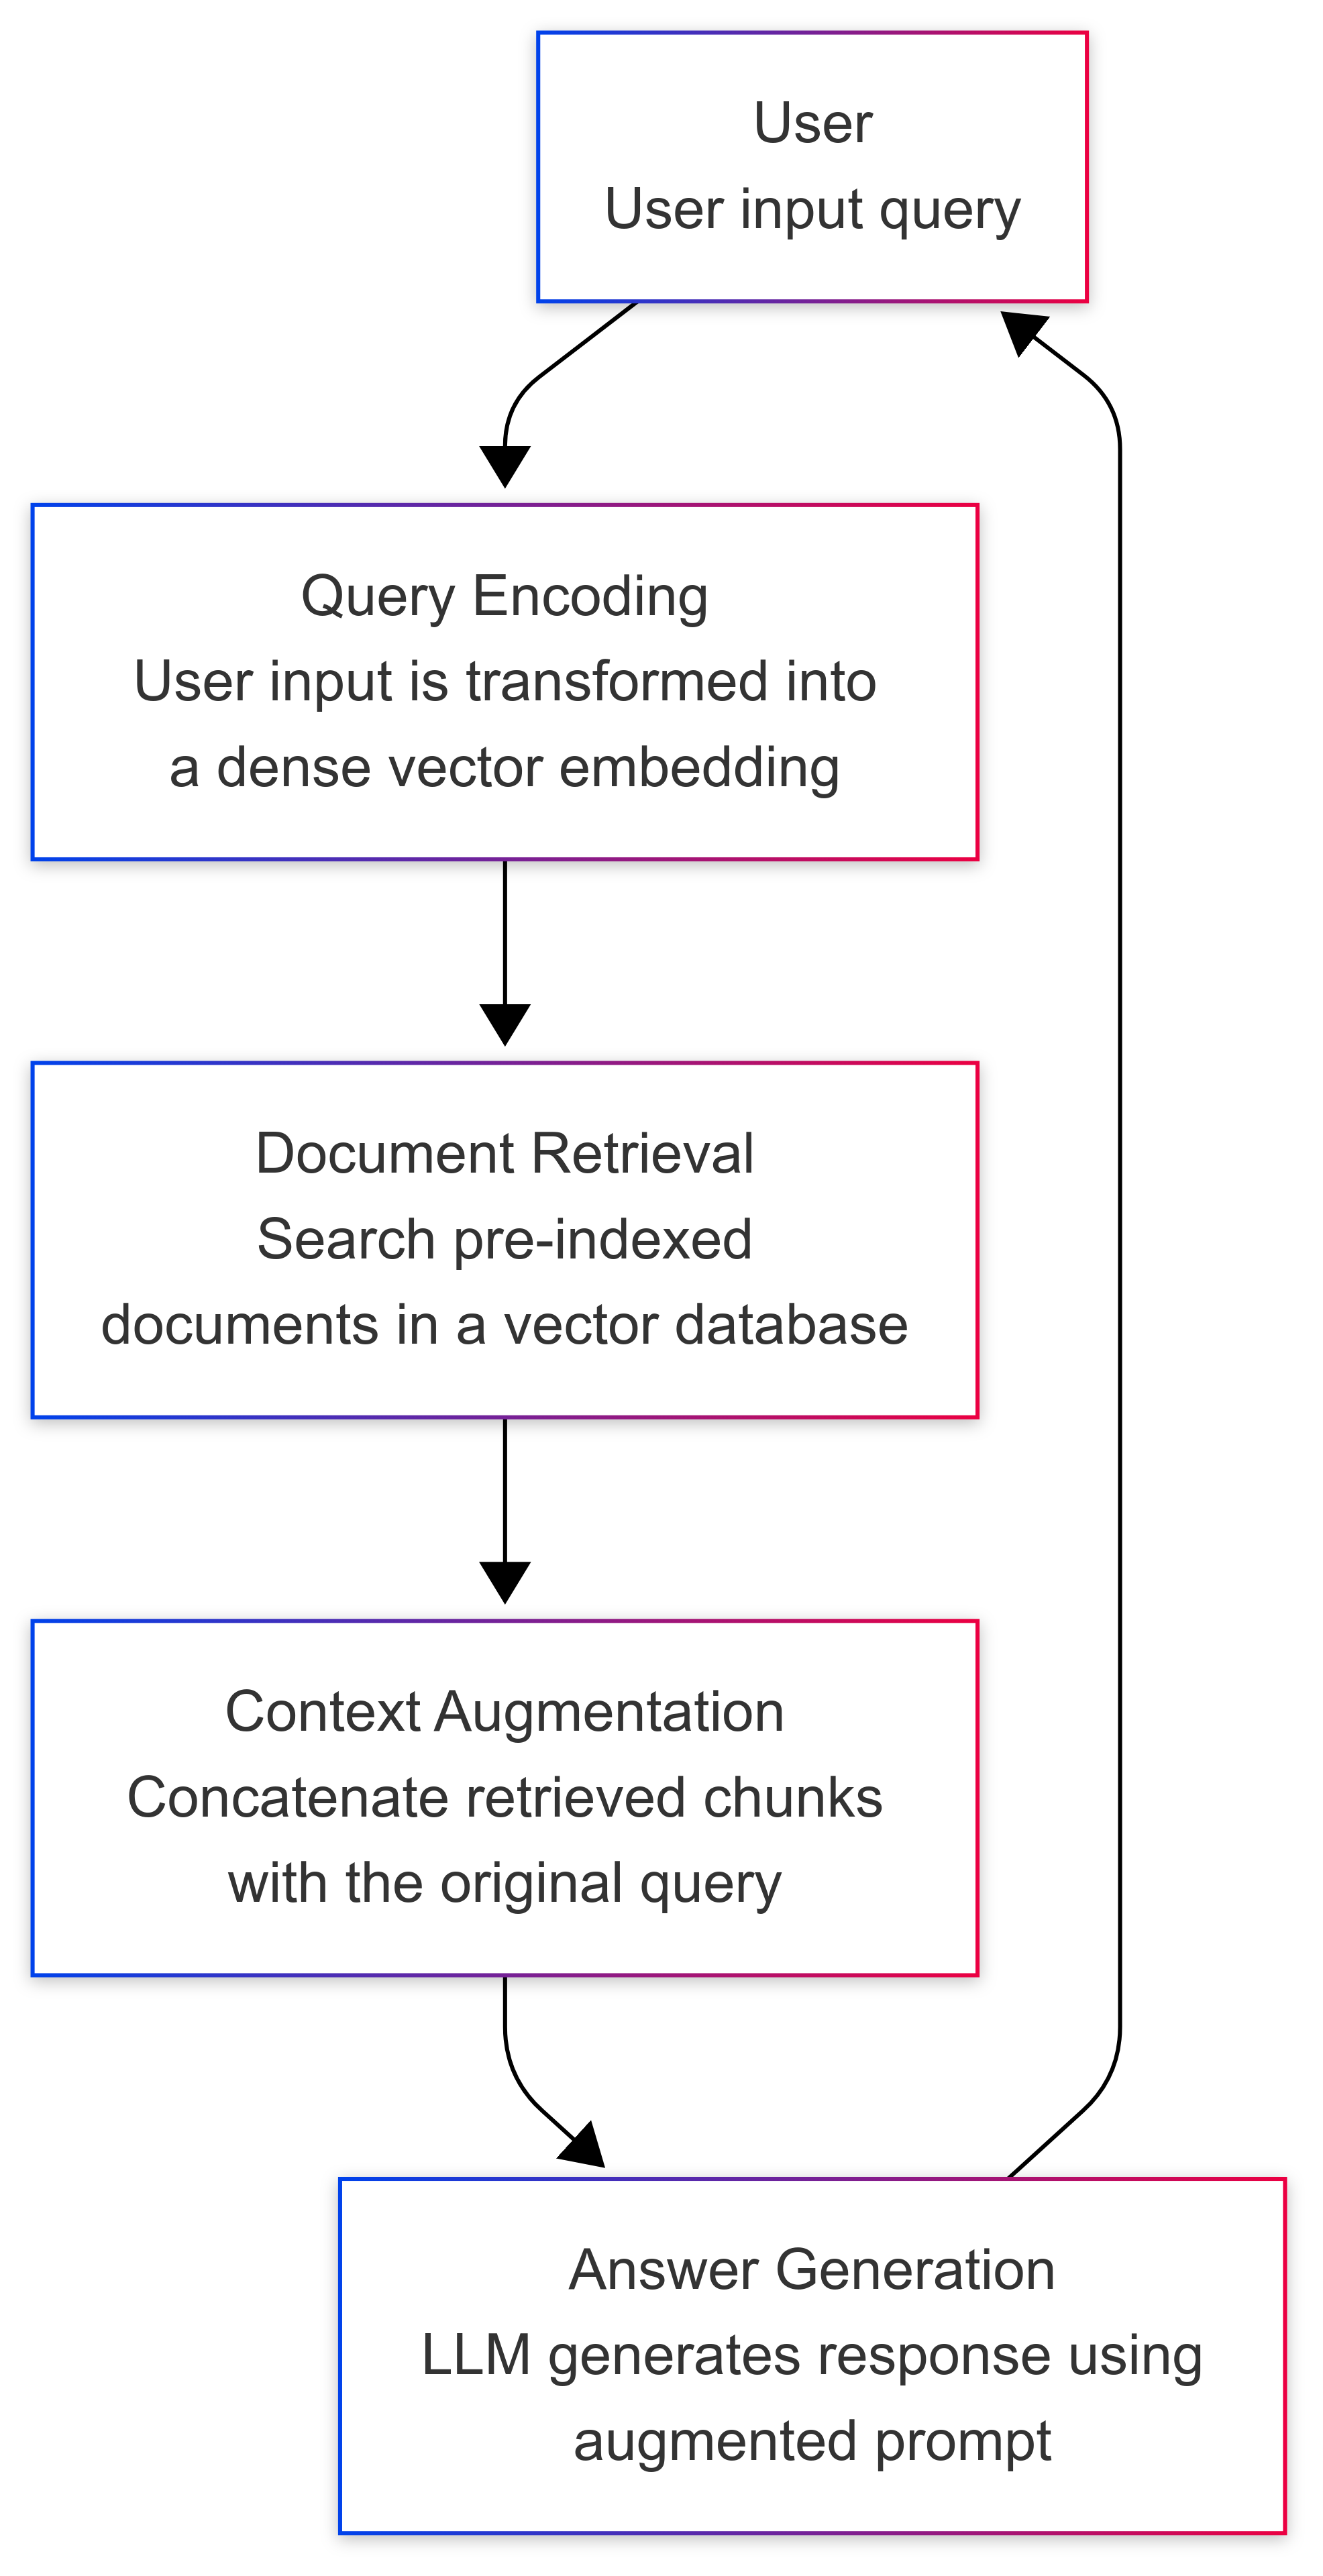
\includegraphics[width=0.3\textwidth]{images/1/rag-pipeline.png}
    \caption{The typical RAG pipeline.}
    \label{fig:rag-pipeline}
\end{figure}

The \textbf{benefits of RAG} anre manifold. it significantly reduces the likelihood of "hallucinations" by anchoring responses to factual data retrieved from the external knowledge base~\cite{xu2025simragselfimprovingretrievalaugmentedgeneration}.
RAG systems can access up-to-date information without the need for frequent and costly retraining of the entire LLM; the knowledgebase can be updated independently. This also enables domain specialization by simply providing a domain-spesific knowledge base. Furthermore, RAG can facilitate source attribution, allowing users to verify the information presented in the LLM's response by referring to the source documents.

RAG implementation can range from simple (Naive RAG) to more complex (Advanced RAG) techniques~\cite{gao2024retrievalaugmentedgenerationlargelanguage}:

\begin{itemize}
    \item \textbf{Naive RAG:} The most basic RAG approach, which simply retrieves relevant documents based on query similarity from the knowledge base and uses them as context for the LLM's response generation.
    \item \textbf{Advanced RAG:} This approach incorporates additional techniques at various stages of the RAG pipeline to improve performance:
    \begin{itemize}
      \item \textbf{Pre-Retrieval Strategies:} Techniques like query expansion(e.g., adding synonyms or related terms), query transformation(e.g., rephrasing the query for clarity), or generating multiple sub-queries from a complex query to retrieve a richer set of documents.
      \item \textbf{Retrieval Strategies:} Moving beyond simple dense vector retrieval to include hybrid search (combiningn keyword-based search like BM25 with semantic search), optimizing the choise and fine-tuning of embedding models, or employing graph-based retrieval mechanisms (e.g., Graph RAG, KG-RAG, where knowledge graphs are used to enhance retrieval).
      \item \textbf{Post-Retrieval/Re-rangking:} After an initial set of documents is retrieved (e.g., top-N candidates), a re-rangking model is used to to re-order these documents based on a more fine-grained assessment of their relevance to the query~\cite{Ma_2023}. Cross-encoder models, which joinly process the query and each candidate document, are often effective for this but are computationally expensive than bi-encoder retrievers.
      \item \textbf{Iterative/Multi-hop Retrieval:} For complex questions that require synthesizing information from multiple sources or performing multi-step reasoning, iterative retrieval techniques can be employed. This might involve decomposing the main question into sub-questions, retrieving evidence for each, and then synthesizing an answer~\cite{jin2025searchr1trainingllmsreason}. The Collab-RAG framework, for example, proposes using smaller language model (SLM) to decompose complex queries, with a larger LLM acting as the reader/synthesizer.
      \item \textbf{Fine-tuning RAG Components:} This involves training the retriever (embedding model) and/or the generator LLM spesifically for the RAG task and target domain. This can improve the alignment between the retriever and generator and enhance the generator's ability to utilize retrieved context effectively~\cite{xu2025simragselfimprovingretrievalaugmentedgeneration}.
    \end{itemize}
\end{itemize}

\textbf{Embedding models} play a crucial role in the RAG pipeline, as they are responsible for converting text (queries and documents) into dense vector representations. State-of-the-art embedding models include Google's Gemini Embedding (models like text-embedding-004 and the experimental gemini-embedding-exp-03-07), which has shown top performance on the MTEB Multilingual benchmark~\cite{kilpatrick2025gemini}.

Other strong open-source multilingual models like multilingual-e5-large-instruct are also widely used. The performance of these models is often evaluated on benchmarks like MTEB (Massive Text Embedding Benchmark)~\cite{muennighoff2023mtebmassivetextembedding} and its multilingual extension, MMTEB~\cite{enevoldsen2025mmtebmassivemultilingualtext}, which cover various tasks and
languages. For Indonesian, specific resources like the Indonesian Sentence Embeddings project and its associated benchmarks (e.g., SemRel2024, Indonesian subsets of MIRACL and TyDiQA) provide valuable evaluation points~\cite{wongso2024indonesian}

The generated embeddings are typically stored and queried using \textbf{vector databases}. Theses databases are optimized for efficient similarity search in high-dimensional spaces, employing Approximate Nearest Neighbor (ANN) algorithms  like HNSW (Hierarchical Navigable Small World)~\cite{malkov2018efficientrobustapproximatenearest} or IVF (Inverted File Index)~\cite{chirkin2024ivfpq}. Key features to consider when choosing a vector database include scalability, query latency, support for metadata filtering (allowing hybrid search), and ease of integration. Popular open-source options suitable for academic research include FAISS, Milvus, and Qdrant~\cite{payong2024choosing}.

Despite its advantages, RAG systems face several challenges:

\begin{itemize}
    \item \textbf{Retrieval Quality:} The "garbage in, garbage out" principle applies; if the retriever fails to fetch relevant documents or retrieves low-quality information, the generator's output will likely be inaccurate or irrelevant. A common issue is the "lost in the middle" problem, where LLMs tend to ignore relevant information if it's buried within a long contextn of retrieved documents~\cite{Zhang2025}.
    \item \textbf{Generation Quality:} Even with relevant retrieved documents, the LLM might still hallucinate, fail to synthesize information coherently from multiple documents, or produce responses that are not faithful to the provided sources~\cite{10.1145/3644815.3644945,zhou2024trustworthinessretrievalaugmentedgenerationsystems}.
    \item \textbf{Context Window Limitations:} LLMs have a finite input context windows. Effectively summarizing and presenting a large amount of retrieved information to LLM without exceeding this limit or losign crucial details is a challenge. 
    \item \textbf{Evaluation Complexity:} Evaluating a multi-stage RAG pipeline ins inherently complex, as it requires assessing the the performance of both the retrieval abd generation components, as well as their interaction~\cite{brehme2025llmstrustedevaluatingrag}.
    \item \textbf{Safety and Bias:} RAG systems can inadvertently propagate biases present in the retrieved documents. There's also a risk that even if the retrieved documents are safe and factual, a non-safety-aligned LLM might still misinterprete or "twist" this information to generate unsafe or misleading outputs~\cite{an2025ragllmssafersafety}.
\end{itemize}

Given the nature of Indonesian consular information—which often involves legal nuances, specific procedural details, and varying citizen situations—a naive RAG approach may prove insufficient. The complexity and criticality of providing accurate consular advice necessitate the exploration and implementation of advanced RAG techniques. Specifically, effective re-ranking of retrieved documents to ensure high relevance, and potentially iterative retrieval strategies for handling complex, multi-faceted queries, will be crucial for building a robust and reliable system.
Furthermore, the inherent limitations of the SahabatAI model, such as its potential for
hallucination, can be better mitigated by providing it with higher quality, more
precisely retrieved context that advanced RAG components can offer.

\section{Fine-tuning LLMs for Domain-Specific QA and RAG}

Fine-tuning pre-trained LLMs is a critical step in adapting then to spesific domains or task, such as the nuanced requirements of consular questions answering. This process adjusts the model's paramaters using a smaller, domain-specific dataset, enabling it to learn the particular vocabulary, style, and knowledge patterns relevant to the target application.

A distincion is made between \textbf{Full Fine-Tuning (FFT)} and \textbf{Parameter-Efficient Fine-Tuning (PEFT)}:

\begin{itemize}
    \item \textbf{Full Fine-Tuning (FFT):} This approach involves updating all parameters of the pre-trained model during the fine-tuning process. While effective, it is computationally expensive, requires significant memory resources, making it less practical for large models or limited hardware environments. it also requires large domain-specific datasets to avoid overfitting. A notable drawback is the risk of "catastrophic forgetting," where the model loses some of its general capabilities learned during pre-training.
    \item \textbf{Parameter-Efficient Fine-Tuning (PEFT):} PEFT methods aim to overcome the limitations of FFT by only updating a small subset of parameters or introducing additional lightweight modules while keeping the majority of the model's parameters frozen. This approach significantly reduces the computational burden and memory requirements, making it feasible to fine-tune large models on smaller datasets. Popular PEFT techniques include:
    \begin{itemize}
      \item \textbf{LoRA (Low-Rank Adaptation) and QLoRA (Quantized LoRA):} LoRA introduces small, trainable low-rank matrices into the layers of the transformer model, effectively learning task-specific adaptations altering the original weights~\cite{hu2021loralowrankadaptationlarge}. QLoRA extends this by quantizing the model weights (e.g., to 4-bit precision) to further reduce memory usage and computational cost~\cite{dettmers2023qloraefficientfinetuningquantized}. QLoRA has proven particularly effective for fine-tuning Gemma-based models~\cite{gemma_qlora_2025}
      \item \textbf{Adapter Layers:} These involve inserting small, trainable neural network modules (adapters) between the existing layers of the pre-trained model. During fine-tuning, only the adapter parameters are updated, while the original model parameters remain frozen~\cite{hu2023llmadaptersadapterfamilyparameterefficient}.
      \item \textbf{Prefix Tuning:} This method adds a small set of trainable prefix tokens to the input sequence. The model learns to modulate its behavior based on these learned prefixes, without changing the core LLM parameters~\cite{li-liang-2021-prefix}.
    \end{itemize}
\end{itemize}

Instruction Fine-Tuning (IFT) is a specific type of fine-tuning that trains LLMs on datasets composed of (instruction, input, output) triplets. This helps the model learn to follow instructions better and perform specific tasks as directed. for QA tasks, this typically involves fine-tuning on (questions, context, answer) examples. In the context of RAG, IFT can be applied to:

\begin{itemize}
    \item Fine-tune the generator LLM to improve its ability to generate accurate and relevant answers based on the retrieved context or adhere to specific formatting requirements.
    \item Jointly train the retriever and generator components to improve their alignment and overall RAG performance.
    \item \textbf{RuleRAG:} is an example where symbolic rules are introduced as demonstration for in-context learning or as part of supervised fine-tuning data to explicitly guide both the retriever (to fetch logically related documents) and the generator (to produce answers that follow the rules)~\cite{chen2025ruleragruleguidedretrievalaugmentedgeneration}.
    \item \textbf{Join QA and Question Generation(QG):} Some research explores fine-tuning an LLM to perform both QA and QG tasks, allowing the model to generate questions based on the retrieved context and then answer them. This can enhance the model's understanding of the context and improve its ability to generate relevant answers~\cite{xu2025simragselfimprovingretrievalaugmentedgeneration}.
\end{itemize}

A crucial consideration in fine-tuning is the minimum dataset size required to achieve effective results. Recent studies, such as the LIMA paper~\cite{NEURIPS2023_ac662d74}, as cited in~\cite{ratnakar2025qapairsassessingparameterefficient}, suggest that even small but high-quality datasets (around 1000 samples) can yield significant improvements in performance when using PEFT techniques.
This is because most of the foundational knowledge is already acquired duirng the extensive pre-training phase. This finding makes the creation of suitable fine-tuning dataset for Indonesian consular QA an achieveable goal within the scope of this research.

\textbf{Compared Studies} often explore the trade-offs between fine-tuning alone, RAG alone, or a combination, or a combination of both (FT + RAG)~\cite{balaguer2024ragvsfinetuningpipelines,alghisi2024finetuneragevaluatingdifferent,ovadia2024finetuningretrievalcomparingknowledge}:
\begin{itemize}
    \item \textbf{RAG alone} excels in tasks requiring access to external, up-to-date, or proprietary knowledge. It is generally less prone to hallucination if the retriever is accurate and allows for easier knowledge updates by modifying the vector database rather retraining the LLM.
    \item \textbf{Fine-tuning alone} is effective for teaching the LLM new skils, adapting its style or tone, or instilling deep understanding of specific domain language and nuances. It can lead to higher accuracy on specialized task where the requirend knowledge can be embedded into the model's parameters. However, it risks catastrophic forgetting and the model's knowledge remains static based on its training data cu-off.
    \item \textbf{FT + RAG} is often considered the most effective approach, combining the strengths of boths. Fine-tuning can make the LLM a better reasoner or synthesizer over the contextual information provided by the RAG system. For example, the generator LLM with RAG pipeline can be fine-tuned to better handle the structure of retrieved documents, to follow specific instructions fir answer generation based on the domain's requirements, or to improve its faithfulness to the provided sources.
\end{itemize}

For fine-tuning Gemma-based models like SahabatAI, the QLoRA method is particularly promising. Libraries like Hugging Face Transformers, along with the PEFT and TRL (Transformer Reinforcement Learning) libraries (specifically the SFTTrainer), provide robust tools for implementing QLoRA fine-tuning for Gemma models~\cite{gemma_qlora_2025}. Keras, with backends like JAX, TensorFlow, or PyTorch, also offers support for LoRA tuning of Gemma models~\cite{gemma_lora_2025}.

The selection of QLoRA as the PEFT strategy for SahabatAI in this thesis is well supported by its efficiency with Gemma-based models. Its ability to handle the model's large parameter size, and its effectiveness in improving performance on domain-specific tasks with smaller datasets (around 1000 samples) further strengthens its suitability for this research. 

\section{AI in Government and Consular Services}

The adoption of AI in government and public services has gained momentum in recent years, with numerous countries implementing AI solutions to enhance efficiency, accessibility, and citizen engagement. 
Global Case Studies provide valuable insights into the potential and challenges of AI:
\begin{itemize}
    \item \textbf{Singapore:} Since the launch of AI-powered chatbots like Ask Jamie, HealthBuddy, and the CPF Chatbot in the mid-2010s, Singapore has progressively enhanced its use of AI in public services. These early systems utilized Natural Language Processing (NLP) to handle citizen inquiries across multiple languages, significantly reducing call center workloads and improving response efficiency~\cite{govtech2016askjamie}. Building on this foundation, Singapore has developed more advanced AI tools such as Pair, an AI assistant designed to boost productivity among public officers, and VICA, a conversational AI platform serving over 60 government agencies and handling hundreds of thousands of queries monthly~\cite{govtech2025pair}. Additionally, specialized AI applications like the OneService Chatbot, which routes municipal feedback with about 80\% accuracy, and PEACH, an AI chatbot aiding perioperative clinical decisions with over 96\% accuracy, demonstrate Singapore's commitment to integrating AI for both operational efficiency and domain-specific expertise~\cite{chong2024peach}. Together, these developments illustrate Singapore's trajectory from basic NLP chatbots to sophisticated, large-scale AI deployments driving a smarter, more responsive public sector. \cite{govsgvica2025}.
    \item \textbf{Japan:} Since 2020, Japan has made significant strides in integrating large language models (LLMs) into its healthcare sector. In April 2025, researchers at the National Institute of Informatics developed a generative AI system that successfully passed the national medical licensing examination. Trained on over 700,000 licensed medical papers, 16 million documents from reputable medical websites, and medical textbooks, this LLM is designed to assist clinicians by suggesting potential diagnoses based on patient interviews. The government plans to deploy this model in medical institutions to support clinical decision-making and improve operational efficiency~\cite{nii2025ai,crds2024rwd}
    \item \textbf{European Union:} The \textbf{iBorderCtrl} project,  was an EU-funded initiative under the Horizon 2020 program, running from September 2016 to August 2019. The project aimed to enhance the efficiency and security of land border crossings for third-country nationals entering the Schengen Area. The system introduced a two-stage process: pre-travel registration and on-site border control. However, the iBorderCtrl project faced significant criticism regarding its ethical implications and scientific validity. Concerns were raised about the reliability of AI-based lie detection, potential biases in facial recognition technology, and the risk of infringing on individuals' rights to privacy and fair treatment. A study published highlighted statistical and methodological flaws in the system's design, questioning the effectiveness of using "biomarkers of deceit" for mass screening purposes~\cite{sánchezmonedero2020politicsdeceptivebordersbiomarkers}. 
    \textbf{AskThePublic}, an AI-powered chatbot integrated into the "Have Your Say" platform. This tool allows citizens to interactively explore and contribute to EU policy consultations. By leveraging large language models, AskThePublic provides structured responses and improved language capabilities, thereby increasing public engagement in the policymaking process. A study published in April 2025 highlights its effectiveness in fostering inclusive decision-making and enhancing democratic participation~\cite{sprenkamp2025effectiveeueparticipationdevelopment}.
    The 2022 report AI Watch~\cite{doi/10.2760/39336} provides a comprehensive analysis of AI adoption across EU public administrations. Conducted by the European Commission's Joint Research Centre, the study maps AI use in public services through three main pillars: an analysis of national AI strategies, an inventory of 686 AI use cases across EU Member States, and in-depth case studies. Findings indicate that while a third of AI initiatives are operational, many remain in pilot or development stages. AI applications predominantly support public service engagement, policy analysis, and internal management. The report emphasizes that successful AI adoption is driven by national governments' capacity and highlights the significant role of regional and local administrations. It also underscores challenges such as data governance, technical capacity, and ethical considerations, advocating for a responsible and inclusive approach to AI integration in the public sector.
    \item \textbf{United States:} The U.S. federal government has significantly expanded its use of artificial intelligence (AI) across public services, aiming to enhance efficiency, decision-making, and service delivery~\cite{ncsl2024ai}. As of 2024, agencies reported 1,757 AI use cases, more than doubling the previous year's count. Notable implementations include the U.S. Patent and Trademark Office employing AI to streamline patent classification, the State Department utilizing AI for document translation and policy summarization, and the Transportation Security Administration integrating AI to expedite airport screenings~\cite{brookings2024ai} . To ensure responsible AI adoption, the Office of Management and Budget (OMB) issued policy M-24-10, mandating agencies to designate Chief AI Officers, implement risk management practices, and enhance transparency in AI applications\cite{OMB-M-24-10}.
    
    Despite these advancements, challenges persist. The Government Accountability Office (GAO) identified that many agencies have yet to fully comply with federal AI requirements, such as maintaining comprehensive AI inventories and updating workforce classifications to include AI competencies. The GAO recommended that 19 agencies take corrective actions to align with established AI policies and guidance~\cite{gao2024ai} . Additionally, the National Conference of State Legislatures (NCSL) reported that over 30 states have issued AI-related guidance, focusing on ethical frameworks, oversight, and pilot projects to guide AI integration at the state level~\cite{ncsl2024ai}

    \item \textbf{Indonesia:} Guided by the National AI Strategy (2020-2045), Indonesia has been actively exploring the integration of AI in public services. This strategy prioritizes five key sectors: health,bureaucratic reform , education and research, food security, mobility and smart cities~\cite{stranaska,desouza2024ai}. Several AI implementations have emerged across Indonesia. In Surabaya, an AI-driven traffic management system employs computer vision to process live CCTV footage, enabling dynamic traffic control that helps alleviate congestion and lower emissions. In West Java, AI technologies support disease surveillance and outbreak forecasting by analyzing a variety of data sources to detect potential hotspots and facilitate timely public health interventions. Meanwhile, Badung Regency in Bali has introduced an AI-powered virtual assistant that uses natural language processing to offer personalized guidance and support to tourists, thereby enhancing visitor experience and contributing to the local economy.~\cite{headfoundation2024inai}.
    To assess its readiness for AI integration, Indonesia collaborated with UNESCO to complete the AI Readiness Assessment, marking it as the first Southeast Asian country to do so. The assessment, involving over 500 participants across five regions, evaluated the country's AI landscape across legal, socio-cultural, economic, educational, and infrastructural dimensions. Findings highlighted the need for ethical AI governance, infrastructure development, and capacity building to ensure inclusive and responsible AI adoption~\cite{unescoina2024ai}.

    The Indonesian government is actively pursuing the integration of Artificial Intelligence (AI) into various public sectors, guided by its National Strategy for Artificial Intelligence 2020-2045 \cite{mfat_indonesia_ai_strategy_2023, investjakarta_ai_global_trends_2025}. This strategy prioritizes AI development in key areas including healthcare, bureaucratic reform, education and research, food security, and mobility and smart cities \cite{mfat_indonesia_ai_strategy_2023}. For instance, the government plans to launch an AI application in August 2025 to bolster food security and social protection programs \cite{techinasia_indonesia_ai_2025}, alongside developing AI-based health screening services to improve healthcare accessibility \cite{govinsider_navigating_ai_2025}. The Ministry of Communication and Digital Affairs (Kominfo) is spearheading efforts in AI governance, issuing ethical guidelines for AI use and working on more comprehensive regulations to ensure responsible AI adoption \cite{opengovasia_indonesia_ai_strategy_2025, govinsider_navigating_ai_2025}. Furthermore, the National Research and Innovation Agency (BRIN) has established an AI and Cybersecurity Research Centre and is involved in drafting AI-related presidential regulations \cite{opengovasia_indonesia_ai_strategy_2025}. 
    
    Several concrete examples of AI implementation are emerging. The Ministry of Finance has launched "Coretax," an AI-supported system aimed at automating and integrating core tax administration processes \cite{dipstrategy_fenomena_penerapan_ai}. In a different application, Soekarno-Hatta Airport has introduced AI-powered assistants for immigration communication services \cite{dipstrategy_fenomena_penerapan_ai}. Despite these advancements, Indonesia faces challenges such as bridging the digital talent gap, ensuring adequate digital infrastructure across its vast archipelago, and navigating budgetary constraints for technological adoption \cite{govinsider_navigating_ai_2025, mfat_indonesia_ai_strategy_2023}. The government acknowledges these hurdles and emphasizes a socio-technical approach, focusing on developing digital talent, fostering public-private partnerships, and creating a robust regulatory framework to maximize AI's benefits while mitigating potential risks \cite{govinsider_navigating_ai_2025, opengovasia_indonesia_ai_strategy_2025}.


    
\end{itemize}

\newpage

% Chapter 3: Methodology
\chapter{Methodology}
\section{Research Design}
Outline the research design, including the type of study (e.g., experimental, observational) and the methods used to collect and analyze data.
\section{Data Collection}
Describe how you collected data for your research, including any surveys, interviews, or experiments conducted.
\begin{figure}
    \centering
    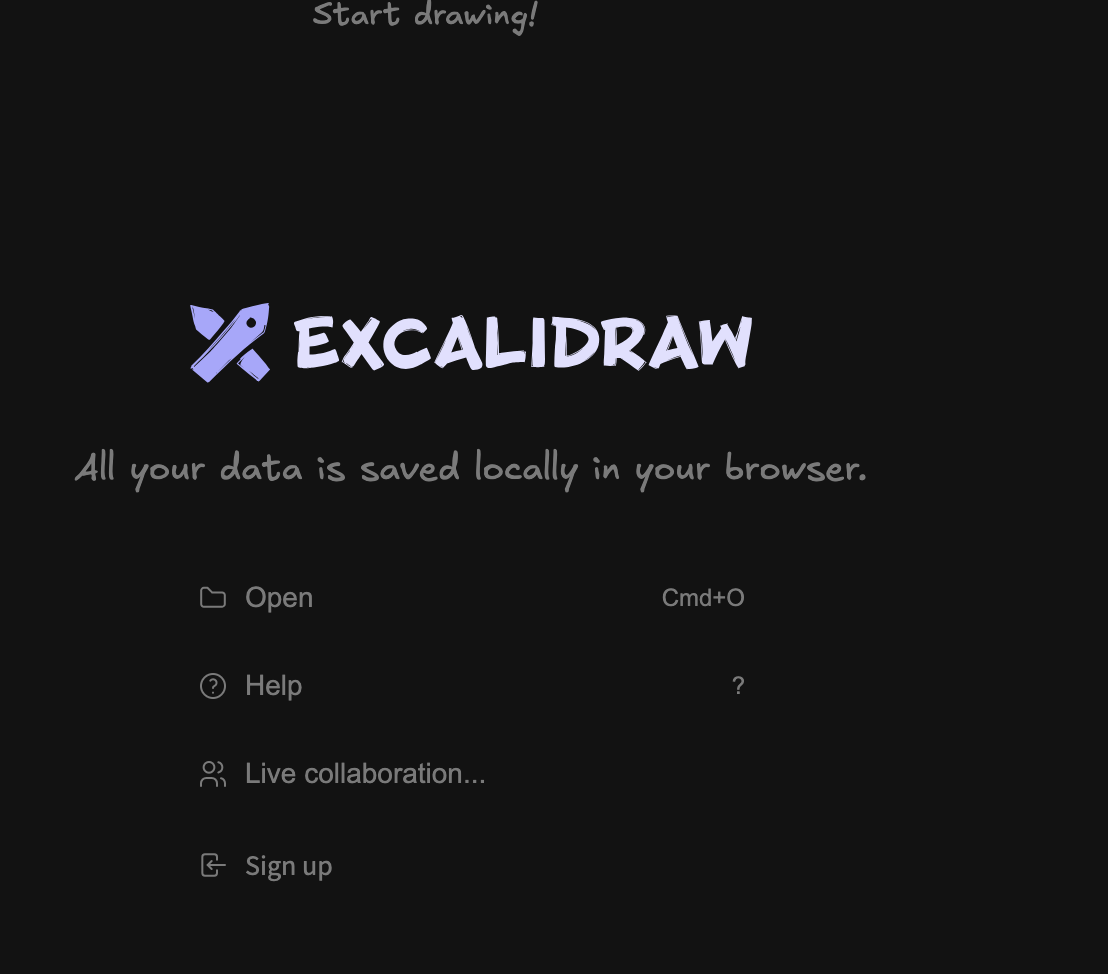
\includegraphics[width=0.8\textwidth]{images/1/apa-ini.png}
    \caption{The typical RAG pipeline.}
    \label{fig:example2}
\end{figure}

\lipsum[1-2] % Dummy text for illustration

\begin{table}[htbp]
  \centering
  \caption{Example of a table caption.}
  \label{tab:example1}
  \begin{tabular}{|l|c|r|}
    \hline
    Column 1 & Column 2 & Column 3 \\
    \hline
    Data A   & 123      & X \\
    Data B   & 456      & Y \\
    Data C   & 789      & Z \\
    \hline
  \end{tabular}
\end{table}

\begin{table}[htbp]
  \centering
  \caption{Example of a table caption.}
  \label{tab:example2}
  \begin{tabular}{lcr}
    \toprule
    Column 1 & Column 2 & Column 3 \\
    \midrule
    Data A   & 123      & X \\
    Data B   & 456      & Y \\
    Data C   & 789      & Z \\
    \bottomrule
  \end{tabular}
\end{table}

\section{Data Analysis}
Explain the methods used to analyze the data, including any statistical tests or software used.
\section{Implementation}
Describe how you implemented the proposed system, including any algorithms or models used.
\section{Evaluation}
Explain how you evaluated the performance of your system, including any metrics used to measure accuracy, precision, recall, etc.
\section{Ethical Considerations}
Discuss any ethical considerations related to your research, including data privacy, consent, and potential biases in the model.

\newpage
% Chapter 4: Results and Discussion
\chapter{Results and Discussion}
Present the results of your research, along with discussions on the implications and findings.

\chapter{Conclusion}
Summarize the key findings of your research and suggest future work or improvements.

\newpage
% References
\sloppy
\printbibliography
\newpage

% Appendices
\appendix
\chapter{Additional Information}
Include any additional data, charts, or detailed explanations that are important for understanding your research.

\end{document}